\documentclass[tikz]{standalone}
\usepackage{fourier}
\usepackage{tikz}

\begin{document}
	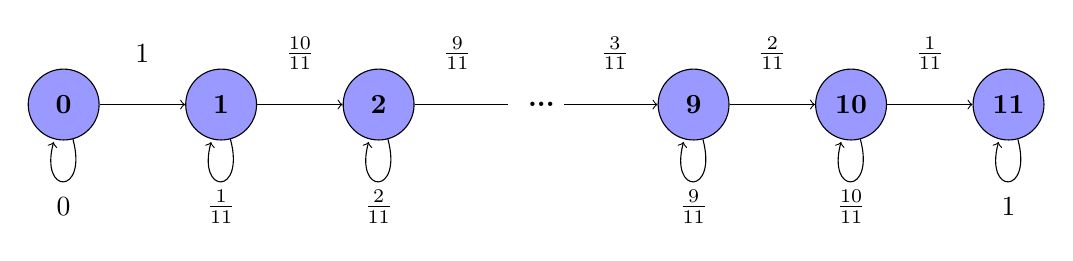
\begin{tikzpicture}
		\node[draw,circle,fill=blue!40!white,minimum size=0.9cm](0) at (0,0) {\textbf{0}};
		\node[draw,circle,fill=blue!40!white,minimum size=0.9cm](1) at (2,0) {\textbf{1}};
		\node[draw,circle,fill=blue!40!white,minimum size=0.9cm](2) at (4,0) {\textbf{2}};
		\node[draw=none](dots) at (6,0) {\textbf{ ... }};
		\node[draw,circle,fill=blue!40!white,minimum size=0.9cm](9) at (8,0) {\textbf{9}};
		\node[draw,circle,fill=blue!40!white,minimum size=0.9cm](10) at (10,0) {\textbf{10}};
		\node[draw,circle,fill=blue!40!white,minimum size=0.9cm](11) at (12,0) {\textbf{11}};
		\node[draw=none] at (0,-1.3) {$0$};
		\node[draw=none] at (2,-1.3) {$\frac{1}{11}$};
		\node[draw=none] at (4,-1.3) {$\frac{2}{11}$};
		\node[draw=none] at (8,-1.3) {$\frac{9}{11}$};
		\node[draw=none] at (10,-1.3) {$\frac{10}{11}$};
		\node[draw=none] at (12,-1.3) {$1$};
		\node[draw=none] at (1,0.65) {$1$};
		\node[draw=none] at (3,0.65) {$\frac{10}{11}$};
		\node[draw=none] at (5,0.65) {$\frac{9}{11}$};
		\node[draw=none] at (7,0.65) {$\frac{3}{11}$};
		\node[draw=none] at (9,0.65) {$\frac{2}{11}$};
		\node[draw=none] at (11,0.65) {$\frac{1}{11}$};
		\draw[->] (0)--(1);
		\draw[->] (1)--(2);
		\draw (2)--(dots);
		\draw[->] (dots)--(9);
		\draw[->] (9)--(10);
		\draw[->] (10)--(11);
		\draw[->] (0) edge [loop below] ();
		\draw[->] (1) edge [loop below] ();
		\draw[->] (2) edge [loop below] ();
		\draw[->] (9) edge [loop below] ();
		\draw[->] (10) edge [loop below] ();
		\draw[->] (11) edge [loop below] ();
	\end{tikzpicture}
\end{document}
